\documentclass[]{article}
\usepackage{graphicx}
\usepackage{amsmath}

%opening
\title{Week 1 Notes}
\author{Uday Manchanda}

\begin{document}

\maketitle

\begin{abstract}
\centering{Week 1 Notes in the Coursera Course on Cryptography}
\end{abstract}

\section{What is Cryptography About?}
\subsection{Course Overview}
\begin{itemize}
	\item Secure communication: HTTPS, WPA2, GSM, Bluetooth, SSL/TLS
	\item SSL/TLS has two main parts:
	\begin{itemize}
		\item Handshake Protocol
		\item Record Layer
	\end{itemize}
	\item Encrypting files on disk: EFS, TrueCrypt
	\item Symmetric Encryption
	\begin{itemize}
		\item 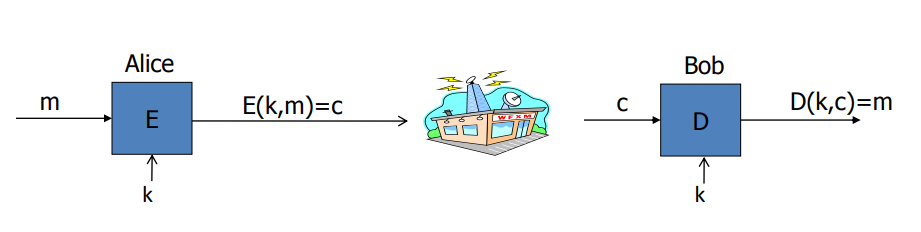
\includegraphics[width=\textwidth]{SymmetricKeyEncryption}
		\item Where:
		\begin{itemize}
			\item E, D: cipher
			\item k : secret key (ex: 128 bits)
			\item m: plaintext
			\item c: ciphertext
		\end{itemize}
		\item Encryption Algorithm is \textbf{publicly known}
	\end{itemize}
	\item Use Cases
	\begin{itemize}
		\item Single use key (one time key)
		\begin{itemize}
			\item key is used to encrypt a single message
			\item new key generated for each email
		\end{itemize}
		\item Multi use key (many time key)
		\begin{itemize}
			\item key encrypts multiple messages
			\item same key used to encrypt many files
		\end{itemize}
	\end{itemize}
\end{itemize}
\subsection{What is Cryptography}
\begin{itemize}
	\item Confidentiality and integrity
	\item Digital signatures, anonymous communication, digital cash
	\item If something can be done with a trusted authority, it can also be done without one
	\item Three steps in cryptography
	\begin{itemize}
		\item Precisely specify threat model
		\item Propose a construction
		\item Prove that breaking construction under threat mode will solve an underlying hard problem
	\end{itemize}
\end{itemize}
\subsection{History}
\begin{itemize}
	\item Substitution cipher
	\begin{itemize}
		\item Find most common letter ("E") via frequencies
		\item Use frequency of pairs of letters
	\end{itemize}
	\item Caesar Cipher
	\begin{itemize}
		\item Shift letters by three
		\item Size of key space: $|\kappa| = 26!$
	\end{itemize}
	\item Vigenere Cipher
	\begin{itemize}
		\item Encrypt message m with some cipher k
		\item For each letter in m, add it to corresponding letter in k
		\item k will "wrap around" until end of message
		\item Take added result and mod 26 to obtain result between 0 and 25
	\end{itemize}
	\item Rotor Machines
	\item Data Encryption Standard (DES)
	\begin{itemize}
		\item keys: $2^{56}$, block size: 64 bits
		\item today AES is in use
	\end{itemize}
\end{itemize}
\section{Discrete Probability}
\subsection{Crash Course Part I}
\begin{itemize}
	\item Let $U$ be some finite set, eg: $U = \{0,1\}^{n}$
	\item Probability distribution P over U is a function $P: U \rightarrow [0,1]$, such that $\sum_{X \in U}^{}P(x) = 1$
	\item EX:
	\begin{itemize}
		\item Uniform Distribution: for all $x \in U: P(x) = \frac{1}{|U|}$
		\item Point Distribution at $x_{0}: P(x_{0}) = 1, \forall x \neq x_{0}: P(x) = 0$
	\end{itemize}
	\item Distribution vector: $( P(000), P(001), P(010), \dots , P(111) )$
	\item Events
	\begin{itemize}
		\item For a set $A \subseteq U: Pr[A] = \sum_{x \in U}^{}P(x) \in [0,1]$
		\item Set A is an \textbf{event}
		\item EX: $U = \{0,1\}^{8}$
		\item A = \{ all x in U such that $lsb_{2}(x) = 11$ \} $\subseteq U$ for the uniform distribution on ${0,1}^{8}: Pr[A] = \frac{1}{4}$
	\end{itemize}
	\item The Union Bound
	\begin{itemize}
		\item For events $A_{1}$ and $A_{2}$: $Pr[A_{1} \cup A_{2}] \leq Pr[A_{1}] + Pr[A_{2}]$
		\item $A_{1} \cap A_{2} = \emptyset \rightarrow Pr[A_{1} \cup A_{2}] = Pr[A_{1}] + Pr[A_{2}]$
		\begin{itemize}
			\item $A_{1} = \{ \text{all x in } {0,1}^{n} \text{ s.t } lsb_{2}(x) = 11 \}$
			\item $Pr[ lsb_{2}(x) = 11 \text{ or } msb_{2}(x) = 11] = Pr[A{1} \cup A_{2}] \leq \frac{1}{4} + \frac{1}{4} = \frac{1}{2}$
		\end{itemize}
	\end{itemize}
	\item Random Variables
	\begin{itemize}
		\item Definition: a random variable X is a function: $X: U \rightarrow V$
		\item EX: $X: \{0,1\}^{n} \rightarrow \{0,1\} ; X(y) = lsb(y) \in \{0,1\}$
		\item For the uniform distribution on U: $Pr[X=0] = \frac{1}{2}, Pr[X=1] = \frac{1}{2}$
		\item more generally: random variable X induces a distribution on V: $Pr[X=v] := Pr[X^{-1}(v)]$
	\end{itemize}
	\item Uniform random variable
	\begin{itemize}
		\item Let U be some set, eg $U = \{0,1\}^{n}$
		\item We write $r \leftarrow U $ to denote a \textbf{uniform random variable} over U for all $a \in U: Pr[r=a] = \dfrac{1}{|U|}$
		\item formally r is the identity function: $r(x) = x \text{for all} x \in U$
		\item Let r be a uniform random variable on $\{0,1\}^{2}$
		\item Define random variable $X = r_{1} + r_{2}$
		\item Then $Pr[X=2] = \dfrac{1}{4}$
		\item Hint: $Pr[X=2] = Pr[r=11]$
	\end{itemize}
	\item Randomized Algorithms
	\begin{itemize}
		\item Deterministic algorithm: $y \leftarrow A(m)$
		\item Randomized algorithm: $y \leftarrow A(m; r)$ where $r \leftarrow \{0,1\}^{n}$
		\item EX: $A(m;k) = E(k,m), y \leftarrow^{n} A(m)$
	\end{itemize}
\end{itemize}
\subsection{Crash Course Part II}
\begin{itemize}
	\item Independence
	\begin{itemize}
		\item Events A and B are \textbf{independent} if $Pr[A \text{ and } B] = Pr[A] \times Pr[B]$
		\item EX: $U = \{0,1\}^{2} = \{00,01,10,11\} and r \leftarrow U$
		\item define r.v X and Y as: $X = \text{ lsb}(r), Y = \text{ msb}(r)$
		\item $Pr[X=0 \text{ and } Y=0 ] = Pr[r=00] = \frac{1}{4} = Pr[X=0] \times Pr[Y=0]$
	\end{itemize}
	\item XOR
	\begin{itemize}
		\item XOR of two strings in $\{0,1\}^{n}$ is their bit-wise addition mod 2
		\item XOR Chart
		\begin{itemize}
			\item (Yeah I made that)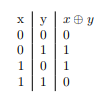
\includegraphics{xor}
		\end{itemize}
		\item EX: $ 0 1 1 0 1 1 1 \oplus 1 0 1 1 0 1 0 = 1 1 0 1 1 0 1$
	\end{itemize}
	\item Important property of XOR
	\begin{itemize}
		\item Theorem: Y a random variable over $\{0,1\}^{n}$, X is an independent uniform variable on $\{0,1\}^{n}$
		\item Then $Z := Y \oplus X$ is a uniform variable on $\{0,1\}^{n}$
		\item Proof for n = 1
		\begin{itemize}
			\item $Pr[Z=0] = Pr[(x,y) = (0,0) \text{ or } (x,y) = (1,1)] $
			\item $Pr[(x,y) = (0,0)] + Pr[(x,y) = (1,1)] = \dfrac{P_{0}}{2} + \dfrac{P_{1}}{2} = \dfrac{1}{2}$
		\end{itemize}
	\end{itemize}
	\item The Birthday Paradox
	\begin{itemize}
		\item Let $r_{1}, \ldots , r_{n} \in U$ be independent indentically distributed random variabes 
		\item When $n = 1.2 \times |U|^{1/2}$ then $Pr[\exists i \neq j : r_{i} = r_{j}] \geq 1/2$
		\item notation: |U| is the size of U
		\item EX: Let $U = \{0,1\}^{128}$
		\begin{itemize}
			\item After sampling about $2^{64}$ random messages from U, some two sampled messages will likely be the same
		\end{itemize}
	\end{itemize}
\end{itemize}
\section{Stream Ciphers}
\subsection{One Time Pad}
\begin{itemize}
	\item Symmetric Ciphers
	\begin{itemize}
		\item Def: a cipher defined over $(K, M, C)$ is a pair of "efficient" algorithms $(E,D)$, where:
		\begin{itemize}
			\item $E = K \times M \rightarrow C$
			\item $D = K \times C \rightarrow M$
			\item $\forall m \in M, k \in K: D(k, E(k,m)) = M $
		\end{itemize}
		\item $E$ is often randomized, $D$ is always deterministic
	\end{itemize}
	\item One Time Pad
	\begin{itemize}
		\item First example of a "secure" cipher
		\item $M = C = \{0,1\}^{n}, K = \{0,1\}^{n}$
		\item key = (random bit string as long as the message)
		\item $C := E(k,m) = k \oplus m$
		\item $D(k,c) = k \oplus c$
		\item $D(k, E(k,m)) = D(k, k \oplus m) = k \oplus (k+m) = (k \oplus k) \oplus m = o \oplus m = m$
		\item You are given a message and its OTP encryption (c). Can you compute the OTP key from m and c?
		\begin{itemize}
			\item Yes, the key is: \textbf{$k = m \oplus c$}
			\item Very fast encryption/decryption...but long keys (as long as plaintext)
		\end{itemize}
	\end{itemize}
	\item What is a secure cipher
	\begin{itemize}
		\item Attacker's abilities: CT only attack (for now)
		\item Possible security attempts
		\begin{itemize}
			\item 1. Attacker cannot recover secret key. $E(k,m) = m $ would be secure
			\item 2. Attacker cannot recover all of the plaintext. $E(k, m_{0} || m_{1}) = m_{0}) || k \oplus m_{1}$ would be secure
			\item Shannon's idea: CT should reveal no "info" about the PT
		\end{itemize}
	\end{itemize}
	\item Information Theoretic security
	\begin{itemize}
		\item Definition: A cipher $(E,D)$ over $(K, M, C)$ has \textbf{perfect secrecy} if:
		\begin{itemize}
			\item $\forall m_{0}, m_{1} \in M, (len(m_{0}) = len(m_{1})), \forall c \in C$
			\item $Pr[E(K, m_{0}) = c] = Pr[E(k, m_{1}) = c]$
			\item where k is uniform in K $(k \leftarrow K)$
			\item Given ciphertext can't tell if message is $m_{0}$ or $m_{1}$ (for all m0, m1)
			\item most powerful adversary learns nothing about plaintext from ciphertext
			\item no ciphertext only attack (other attacks are possible)
		\end{itemize}
		\item Lemma: OTP has perfect secrecy. Proof: 
		\begin{itemize}
			\item $\forall m,c: Pr[E(k,m)=c] = \dfrac{\text{number of keys } \kappa \in K \text{ s.l. } E(k,m)=c}{|K|} $
			\item If $\forall m,c: \text{number} = \{\kappa \in K: E(k,m)=c \} = \text{const}$
			\item Therefore, cipher has perfect secrecy
			\item Let $m \in M $ and $c \in C$. How many OTP keys map m to c? \textbf{one}
			\item However: implies that: $|\kappa| \geq |M| \rightarrow $ hard to use in practice, (key length $>$ message length)
		\end{itemize}
	\end{itemize}
\end{itemize}
\subsection{Pseudorandom Generators}
\begin{itemize}
	\item Stream Ciphers: Making OTP practical
	\begin{itemize}
		\item idea: replace "random" key by "pseudorandom" key
		\item PRG is a function: $G: \{0,1\}^{s} \rightarrow \{0,1\}^{n}$
		\item $n >> s$
		\item computable by a \underline{deterministic} algorithm
		\item $C := E(k,m) = m \oplus G(k)$
		\item $D(k,c) = C \oplus G(k)$
		\item Can a stream cipher have perfect secrecy: No since the key is shorter than the message
		\item Stream ciphers cannot have perfect secrecy
		\begin{itemize}
			\item Need a different definition of security
			\item Security will depend on specific PRG
		\end{itemize}
	\end{itemize}
	\item PRG must be unpredictable
	\begin{itemize}
		\item Suppose PRG is predictable:
		\item $\exists i: G(k) |_{1,...,i} \rightarrow^{alg} G(k) |_{i+1,...,n} $
		\item 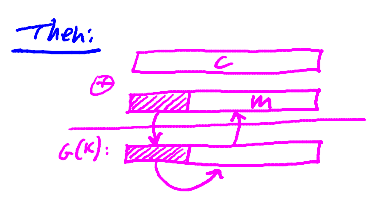
\includegraphics[scale=0.5]{Selection_016}
		\item We say that $G: K \rightarrow \{0,1\}^{n}$ is \textbf{unpredictable} if:
		\begin{itemize}
			\item $\exists \text{ "eff" alg A and } \exists_{0} \leq i \leq n-1 \leq t$
			\item $Pr[A(G(k)) |_{1,...,i} = G(k) |_{i+1}] > \frac{1}{2} + \epsilon$
			\item For non-negligible $\epsilon$, eg $\frac{1}{2^{30}}$
			\item Definition: PRG is unpredictable if it is not predictable, no "efficient" adv. can predict bit (i+1) for "non-neg" $\epsilon$
			\item Suppose $G:K \rightarrow \{0,1\}^{n}$ is such that for all k: $XOR(G(k)) = 1$. Is G predictable? $\rightarrow$ Yes given the first (n-1) bits I can predict the n'th bit
		\end{itemize}
	\end{itemize}
	\item Weak PRGs (do not use for crypto!)
	\begin{itemize}
		\item $\text{glibc random():}$
		\item $		r[i] \leftarrow (r[i-3] + r[i-31]) \% 2^{32}$
		\item $		\text{output } r[i] >> 1$
		\item Never use random() for crypto
	\end{itemize}
\end{itemize}
\subsection{Negligible vs. non-negligible}
\begin{itemize}
	\item Negligible vs. non-negligible
	\begin{itemize}
		\item In practice: $\epsilon$ is a scalar and
		\begin{itemize}
			\item $\epsilon \text{ non-neg } \epsilon \geq \frac{1}{2^{30}}$ (likely to happen over 1 GB of data)
			\item $\epsilon \text { negligible } \epsilon \leq \frac{1}{2^{80}}$ (won't happen over life of key)
		\end{itemize}
		\item In theory: $\epsilon$ is a function: $\epsilon: Z^{\geq 0} \rightarrow R^{\geq 0}$
		\begin{itemize}
			\item $\epsilon \text{ non-neg } \exists d: \epsilon(\lambda) \geq \frac{1}{\lambda^{d}} (\epsilon \geq \frac{1}{poly}, \text{ for many } \lambda) $
			\item $\epsilon \text{ negligible } \forall d, \lambda \geq \lambda_{d}: \epsilon(\lambda) \leq \frac{1}{\lambda^{d}} (\epsilon \leq \frac{1}{poly}, \text{ for large } \lambda) $
		\end{itemize}
		\item Few Examples
		\begin{itemize}
			\item $\epsilon(\lambda) = \frac{1}{2^{\lambda}}$: negligible
			\item $\epsilon(\lambda) = \frac{1}{\lambda^{1000}}$: non-negligible
			\item \[ 
			\begin{cases}
			\frac{1}{2^{\lambda}} & \text{ for odd } \lambda \\
			\frac{1}{\lambda^{1000}} & \text{ for even } \lambda \\
			\end{cases}
			\]
		\end{itemize}
	\end{itemize}
	\item PRGs: the rigorous theory view
	\begin{itemize}
		\item PRGs are parametrized by a security parameter: $\lambda$
		\begin{itemize}
			\item PRG becomes "more secure" as $\lambda$ increases
		\end{itemize}
		\item Seed lengths and output lengths grow with $\lambda$
		\item For every $\lambda=1,2,3,...$ there is a different PRG: $G_{\lambda}$
		\item $G_{\lambda} : K_{\lambda} \rightarrow \{0,1\}^{n(\lambda)}$
		\item We say that the previous equation is \textbf{predictable} at position i if: 
		\begin{itemize}
			\item there exists a polynomial time (in $\lambda$) algorithm A s.t.
			\item $Pr_{k \leftarrow K_{\lambda}} [ A(\lambda, G_{\lambda}(k)) |_{1,...,i} = G_{\lambda}(k) |_{i+1}] > \frac{1}{2} + \epsilon(\lambda)$
			\item For some non-negligible function $\epsilon(\lambda)$
		\end{itemize}
	\end{itemize}
\end{itemize}
\subsection{Attacks on OTP and Stream Ciphers}
\begin{itemize}
	\item Attack 1: Two time pad is insecure
	\begin{itemize}
		\item Never use stream cipher key more than once
		\item $C_{1} \leftarrow m_{1} \oplus PRG(k)$
		\item $C_{2} \leftarrow m_{2} \oplus PRG(k)$
		\item Eavesdropper does: $C_{1} + C_{2} \rightarrow m_{1} \oplus m_{2}$
		\item Enough redundancy in English and ASCII encoding that: $m_{1} \oplus m_{2} \rightarrow m_{1}, m_{2}$
		\item Real World Examples
		\begin{itemize}
			\item Project Venona
			\item MS-PPTP
			\begin{itemize}
				\item Have one key for interaction between server and client
				\item Another one between client and server
			\end{itemize}
			\item 802.11b WEP
			\begin{itemize}
				\item 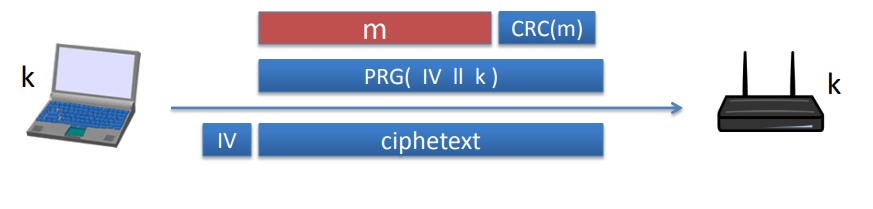
\includegraphics[scale=0.5]{Wep}
				\item Length of IV: 24 bits
				\item Repeated IV after $2^{24} \approx $ 16 M frames
				\item On some 802.11 cards: IV resets to 0 after power cycle
				\item Avoid related keys
			\end{itemize}
			\item Disk encryption (one-time pad does not work)
			\begin{itemize}
				\item As you make changes to a file, the encrypted contents can leak as a hacker can figure out where in memory those changes were made
			\end{itemize}
		\end{itemize}
	\end{itemize}
	\item Attack 2: OTP provides no integrity, is malleable
	\begin{itemize}
		\item (m $\oplus$ k) $\oplus$ p (p is the message used by the hacker)
		\item Decrypting the previous expression will yield m $\oplus$ p
		\item OTP is malleable because it is easy to change ciphertext
	\end{itemize}
\end{itemize}
\subsection{Real World Stream Ciphers}
\begin{itemize}
	\item Old Example 1: RC4
	\begin{itemize}
		\item Input: variable sized seed
		\item Expands into 2048 bits, executes very simple loop to generate one byte/round
		\item Used in HTTPS and WEP
		\item Weaknesses: bias in initial output, probability of (0,0) is $\frac{1}{{256}^{2}} + \frac{1}{{256}^{3}}$, Related key attacks
	\end{itemize}
	\item Old Example 2: CSS(Content Scrambling System)
	\begin{itemize}
		\item Badly broken
		\item Linear feedback shift register
		\begin{itemize}
			\item a register that contains cells
			\item certain taps are in certain cells that feed into an XOR
			\item at every clock cycle register shifts to the left
		\end{itemize}
		\item DVD encryption uses this
		\item seed = 5 bytes
	\end{itemize}
	\item Modern Example: eStream
	\begin{itemize}
		\item PRG: $\{0,1\}^{s} * R \rightarrow \{0,1\}^{n}$
		\item Nonce: a non-repeating value for a given key
		\item First input is a seed, $R$ is the nonce
		\item $E(k, m:r) = m \oplus PRG(k; r)$
		\item the pair $k,r$ is never used more than once
		\item can reuse the key because $(k,r)$ is unique
		\item eStream: Salsa20 (SW + HW)
		\begin{itemize}
			\item 128,256 bit seed
			\item 64 bit nonce
			\item $\{0,1\}^{128 \text{ or } 256} * \{0,1\}^{64} \rightarrow \{0,1\}^{n}$
			\item $\text{Salsa20(k;r)} := H(k, (r,0)) || H(k, (r,1)) || ...$
			\item Expand the states into 64 bytes long
		\end{itemize}
	\end{itemize}
\end{itemize}
	
\end{document}
